%Câu 1 
\begin{ex}%[0H9N3-1]%[Dự án đề kiểm tra Toán khối 10 GK2 NH23-24 - Dot 13 - Xuan Vy Pham]%[THPT Chuyên Lê Quý Đôn - Ninh Thuận]
	Trong mặt phẳng toạ độ $Oxy$, đường thẳng $d \colon \heva{&x=2-2t \\ &y=5+6t}$ có một véc-tơ chỉ phương là
	\choice
	{$\overrightarrow{u}_1=(2;6)$}
	{$\overrightarrow{u}_2=(6;2)$}
	{\True $\overrightarrow{u}_3=(-2;6)$}
	{$\overrightarrow{u}_4=(1;3)$}
	\loigiai{Đường thẳng $d 
		\colon \heva{&x=2-2t \\ &y=5+6t}$ có một véc-tơ chỉ phương là $\overrightarrow{u}_3=(-2;6)$.}
\end{ex}
%Câu 2
\begin{ex}%[0H9N3-1]%[Dự án đề kiểm tra Toán khối 10 GK2 NH23-24 - Dot 13 - Xuan Vy Pham]%[THPT Chuyên Lê Quý Đôn - Ninh Thuận]
	Trong mặt phẳng $Oxy$, điểm nào sau đây thuộc đường thẳng $2x-y+1=0$?	
	\choice
	{$M_1 (2;3)$}
	{$M_2 (4;1)$}
	{$M_3 (-1;5)$}
	{\True $M_4 (0;1)$}
	\loigiai{Vì $2 \cdot 0 -1+1=0$ nên điểm $M_4 (0;1)$ thuộc đường thẳng $2x-y+1=0$.}
\end{ex}
%Câu 3
\begin{ex}%[0H9N3-1]%[Dự án đề kiểm tra Toán khối 10 GK2 NH23-24 - Dot 13 - Xuan Vy Pham]%[THPT Chuyên Lê Quý Đôn - Ninh Thuận]
	Trong mặt phẳng $Oxy$, đường thẳng $\Delta \colon 3x-y+1=0$ có một véc-tơ pháp tuyến là	
	\choice
	{\True$\overrightarrow{n}_1=(3;-1)$}
	{$\overrightarrow{n}_2=(3;1)$}
	{ $\overrightarrow{n}_3=(1;3)$}
	{$\overrightarrow{n}_4=(-1;3)$}
	\loigiai{Đường thẳng $\Delta \colon 3x-y+1=0$ có một véc-tơ pháp tuyến là $\overrightarrow{n}_1=(3;-1)$.}
\end{ex}
%Câu 4 
\begin{ex}%[0H9N3-1]%[Dự án đề kiểm tra Toán khối 10 GK2 NH23-24 - Dot 13 - Xuan Vy Pham]%[THPT Chuyên Lê Quý Đôn - Ninh Thuận]
	Đường thẳng $d$ có một véc-tơ pháp tuyến là $\overrightarrow{n}=(2;-1)$. Trong các véc-tơ sau, véc-tơ nào là một véc-tơ chỉ phương của $d$?	
	\choice
	{$\overrightarrow{u}_1=(1;-2)$}
	{$\overrightarrow{u}_2=(-1;2)$}
	{\True $\overrightarrow{u}_3=(1;2)$}
	{$\overrightarrow{u}_4=(2;1)$}
	\loigiai{Vì đường thẳng $d$ có một véc-tơ pháp tuyến là $\overrightarrow{n}=(2;-1)$ nên nó có một véc-tơ chỉ phương là $\overrightarrow{u}_3=(1;2)$.}
\end{ex}
%Câu 5
\begin{ex}%[0D8H2-1]%[Dự án đề kiểm tra Toán khối 10 GK2 NH23-24 - Dot 13 - Xuan Vy Pham]%[THPT Chuyên Lê Quý Đôn - Ninh Thuận]
	Với $k$, $n$ là hai số tự nhiên tùy ý thỏa mãn $1 \le k \le n$, khẳng định nào sau đây là đúng?	
	\choice
	{\True $\mathrm{A}_n^k=\dfrac{n!}{\left(n-k\right)!}$}
	{$\mathrm{A}_n^k=\dfrac{n!}{k!}$}
	{$\mathrm{A}_n^k=\dfrac{n!}{k!\left(n-k\right)!}$}	{$\mathrm{A}_n^k=\dfrac{k!\left(n-k\right)!}{n!}$}
	\loigiai{Khẳng định đúng là $\mathrm{A}_n^k=\dfrac{n!}{\left(n-k\right)!}$.}
\end{ex}
%Câu 6
\begin{ex}%[0D8H3-4]%[Dự án đề kiểm tra Toán khối 10 GK2 NH23-24 - Dot 13 - Xuan Vy Pham]%[THPT Chuyên Lê Quý Đôn - Ninh Thuận]
	Số hạng tổng quát trong khai triển của biểu thức $(a+b)^4$ là
	\choice
	{\True $T_{k+1}=\mathrm{C}_4^k a^{4-k}b^k$, $0 \le k \le 4$}
	{$T_{k+1}=\mathrm{C}_4^k a^{k}b^k$, $0 \le k \le 4$}
	{$T_{k+1}=\mathrm{C}_4^k a^{4-k}b^{4-k}$, $0 \le k \le 4$}
	{$T_{k+1}=\mathrm{C}_4^k a^{4}b^{4-k}$, $0 \le k \le 4$}
	\loigiai{Số hạng tổng quát trong khai triển của biếu thức $(a+b)^4$ là $T_{k+1}=\mathrm{C}_4^k a^{4-k}b^k$, $0 \le k \le 4$.} 
\end{ex}
%Câu 7
\begin{ex}%[0H9H1-3]%[Dự án đề kiểm tra Toán khối 10 GK2 NH23-24 - Dot 13 - Xuan Vy Pham]%[THPT Chuyên Lê Quý Đôn - Ninh Thuận]
	Trong mặt phẳng $Oxy$, cho $A(2;-3)$, $B(-3;-1)$, $C(4;-2)$. Tọa độ trọng tâm $G$ của $\triangle ABC$ là
	\choice
	{\True $G(1;-2)$}
	{$G(3;-6)$}
	{$G(2;-4)$}
	{$G(2;-2)$}
	\loigiai{Vì $G$ là trọng tâm của $\triangle ABC$ nên
		$$\heva{&x_G = \dfrac{x_A+x_B+x_C}{3}\\&y_G = \dfrac{y_A+y_B+y_C}{3}} \Leftrightarrow \heva{&x_G = \dfrac{2-3+4}{3}\\&y_G = \dfrac{-3-1-2}{3}} \Leftrightarrow \heva{&x_G=1 \\ &y_G=-2.}$$ 
	Vậy trọng tâm $G$ có tọa độ là $(1;-2)$.}
\end{ex}
%Câu 8
\begin{ex}%[0H9H1-3]%[Dự án đề kiểm tra Toán khối 10 GK2 NH23-24 - Dot 13 - Xuan Vy Pham]%[THPT Chuyên Lê Quý Đôn - Ninh Thuận]
	Cho véc-tơ $\overrightarrow{c}$ được biểu diễn trong mặt phẳng tọa độ $Oxy$ như hình vẽ dưới đây
	\begin{center}
		{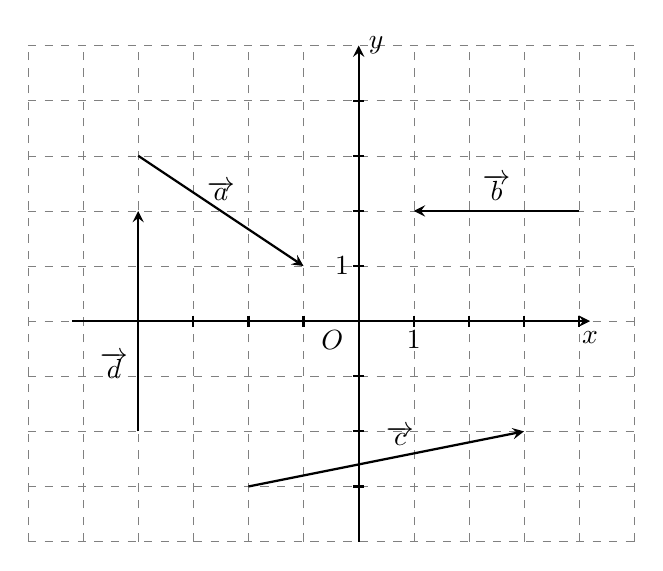
\begin{tikzpicture}[x=0.7 cm,y=0.7 cm,>=stealth]
				%Vẽ lưới
				\draw[step=1,gray,dashed,very thin]
				(-6,-4) grid (5,5);
				% Tiến hành vẽ hai trục tọa độ
				\draw[->, color=black, thick] (-5.2,0) -- (4.2,0) node[below] {$x$};
				\foreach \x in 	{-4,-3,-2,-1,1,2,3,4}
				\draw[shift={(\x,0)},color=black,thick] (0pt,2pt) -- (0pt,-2pt) ;
				\draw[->,color=black,thick] (0,-4) -- (0,5) node[right]{$y$};
				\foreach \y in 	{-3,-2,-1,1,2,3,4}
				\draw[shift={(0,\y)},color=black,thick] (2pt,0pt) -- (-2pt,0pt) ;
				\draw (-0.1,0) node[below left] {$O$};
				\draw[->,thick] (-4,3)--(-1,1) node [pos=0.5,above]{$\overrightarrow{a}$};
				\draw[->,thick] (-2,-3)--(3,-2) node [pos=0.55,above]{$\overrightarrow{c}$};
				\draw[->,thick] (4,2)--(1,2) node [pos=0.5,above]{$\overrightarrow{b}$};
				\draw[->,thick] (-4,-2)--(-4,2) node [pos=0.3,left]{$\overrightarrow{d}$};
				%Vẽ các điểm
				\draw (1,0) node[below]{1};
				\draw (0,1) node[left]{1};
		\end{tikzpicture}}
	\end{center}
	Hãy xác định tọa độ của véc-tơ $\overrightarrow{c}$.	
	\choice
	{$\overrightarrow{c}=(1;5)$}
	{\True $\overrightarrow{c}=(5;1)$}
	{$\overrightarrow{c}=(-1;-5)$}
	{$\overrightarrow{c}=(-5;-1)$}
	\loigiai{Véc-tơ $\overrightarrow{c}$ có điểm đầu có tọa độ là $(-2,-3)$ và điểm cuối có tọa độ là $(3,-2)$ nên tọa độ véc-tơ $\overrightarrow{c}$ là $(3-(-2);(-2)-(-3))=(5;1)$.}
\end{ex}
%Câu 9
\begin{ex}%[0H9H3-3]%[Dự án đề kiểm tra Toán khối 10 GK2 NH23-24 - Dot 13 - Xuan Vy Pham]%[THPT Chuyên Lê Quý Đôn - Ninh Thuận]
	Xác định vị trí tương đối giữa hai đường thẳng $\Delta \colon 2x-y+2023=0$ và $d \colon 4x-2y+2024=0$.	
	\choice
	{$d_1$ và $d_2$ cắt nhau nhưng không vuông góc}
	{$d_1 \equiv d_2$}
	{\True $d_1 \parallel d_2$}
	{$d_1 \perp d_2$}
	\loigiai{Ta có $\dfrac{2}{4}=\dfrac{-1}{-2} \neq \dfrac{2023}{2024}$ nên $d_1$ và $d_2$ song song.}
\end{ex}
%Câu 10
\begin{ex}%[0D8N2-1]%[Dự án đề kiểm tra Toán khối 10 GK2 NH23-24 - Dot 13 - Xuan Vy Pham]%[THPT Chuyên Lê Quý Đôn - Ninh Thuận]
	Công thức tính số tổ hợp chập $3$ của $10$ phần tử là	
	\choice
	{$\mathrm{C}_{10}^3=10!$}
	{$\mathrm{C}_{10}^3=\dfrac{10!}{(10-3)!}$}
	{\True $\mathrm{C}_{10}^3=\dfrac{10!}{3!(10-3)!}$}
	{$\mathrm{C}_{10}^3=3!$}
	\loigiai{Số tổ hợp chập $3$ của $10$ phần tử là $\mathrm{C}_{10}^3=\dfrac{10!}{3!(10-3)!}$.}
\end{ex}
%Câu 11 
\begin{ex}%[0D8N2-1]%[Dự án đề kiểm tra Toán khối 10 GK2 NH23-24 - Dot 13 - Xuan Vy Pham]%[THPT Chuyên Lê Quý Đôn - Ninh Thuận]
	Cho tập hợp $X$ có $n$ phần tử $(n \in \mathbb{N}^*)$, số hoán vị $n$ phần tử của tập hợp $X$ là	
	\choice
	{\True $n!$}
	{$n^2$}
	{$n$}
	{$n^n$}
	\loigiai{Số hoán vị $n$ phần tử của tập hợp $X$ là $n!$.	}
\end{ex}
%Câu 12
\begin{ex}%[0D8H3-2]%[Dự án đề kiểm tra Toán khối 10 GK2 NH23-24 - Dot 13 - Xuan Vy Pham]%[THPT Chuyên Lê Quý Đôn - Ninh Thuận]
	Khai triển Newton biểu thức $(x+2)^5$ ta được	
	\choice
	{\True $(x+2)^5=\mathrm{C}_5^0 x^5 + 2\mathrm{C}_5^1x^4+ 2^2\mathrm{C}_5^2x^3+2^3\mathrm{C}_5^3x^2+2^4\mathrm{C}_5^4x+2^5\mathrm{C}_5^5$}
	{$(x+2)^5=\mathrm{C}_5^0 x^5 - 2\mathrm{C}_5^1x^4+ 2^2\mathrm{C}_5^2x^3-2^3\mathrm{C}_5^3x^2+2^4\mathrm{C}_5^4x-2^5\mathrm{C}_5^5$}
	{$(x+2)^5=\mathrm{C}_5^0 x^5 + 2\mathrm{C}_5^1x^4+ 2^2\mathrm{C}_5^2x^3-2^3\mathrm{C}_5^3x^2+2^4\mathrm{C}_5^4x-2^5\mathrm{C}_5^5$}
	{$(x+2)^5=2\mathrm{C}_5^0 x^5 + 2^2\mathrm{C}_5^1x^4+ 2^3\mathrm{C}_5^2x^3+2^4\mathrm{C}_5^3x^2+2^5\mathrm{C}_5^4x+2^6\mathrm{C}_5^5$}
	\loigiai{Khai triển Newton biểu thức $(x+2)^5$ ta được	$$(x+2)^5=\mathrm{C}_5^0 x^5 + 2\mathrm{C}_5^1x^4+ 2^2\mathrm{C}_5^2x^3+2^3\mathrm{C}_5^3x^2+2^4\mathrm{C}_5^4x+2^5\mathrm{C}_5^5.$$ }
\end{ex}
%Câu 13
\begin{ex}%[0H9N1-3]%[Dự án đề kiểm tra Toán khối 10 GK2 NH23-24 - Dot 13 - Xuan Vy Pham]%[THPT Chuyên Lê Quý Đôn - Ninh Thuận]
	Véc-tơ $\overrightarrow{a}=(-4;0)$ được phân tích theo hai véc-tơ đơn vị như thế nào?	
	\choice
	{\True $\overrightarrow{a}=-4\overrightarrow{i}+0\overrightarrow{j}$}
	{$\overrightarrow{a}=0\overrightarrow{i}-4\overrightarrow{j}$}
	{$\overrightarrow{a}=-4\overrightarrow{i}+\overrightarrow{j}$}
	{$\overrightarrow{a}=\overrightarrow{i}-4\overrightarrow{j}$}
	\loigiai{Vì $\overrightarrow{a}$ có tọa độ là $\overrightarrow{a}=(-4;0)$ nên $\overrightarrow{a}=-4 \overrightarrow{i}+0\overrightarrow{j}$.}
\end{ex}
%Câu 14 
\begin{ex}%[0H9N1-3]%[Dự án đề kiểm tra Toán khối 10 GK2 NH23-24 - Dot 13 - Xuan Vy Pham]%[THPT Chuyên Lê Quý Đôn - Ninh Thuận]
	Cho véc-tơ $\overrightarrow{u}=2\overrightarrow{i}-3\overrightarrow{j}$. Tọa độ của véc-tơ $\overrightarrow{u}$ là	
	\choice
	{$(3;2)$}
	{\True $(2;-3)$}
	{$(-3;2)$}
	{$(2;3)$}
	\loigiai{Vì $\overrightarrow{u}=2\overrightarrow{i}-3\overrightarrow{j}$ nên $\overrightarrow{u}$ có tọa độ là $\overrightarrow{u}=(2;-3)$.}
\end{ex}
%Câu 15
\begin{ex}%[0D8H1-6]%[Dự án đề kiểm tra Toán khối 10 GK2 NH23-24 - Dot 13 - Xuan Vy Pham]%[THPT Chuyên Lê Quý Đôn - Ninh Thuận]
	Một hãng thời trang đưa ra một mẫu áo sơ mi mới có bốn màu gồm trắng, xanh, vàng, đen. Mỗi loại có các cỡ S, M, L. Hình dưới đây là sơ đồ hình cây biểu thị các loại áo sơ mi với màu và cỡ áo nói trên. Nếu một cửa hàng muốn mua tất cả các loại áo sơ mi (đủ loại màu và đủ loại cỡ áo) và mỗi loại một chiếc để về giới thiệu thì cần mua tất cả bao nhiêu chiếc áo sơ mi?	
	\begin{center}
		\begin{tikzpicture}[x=0.7 cm,y=0.7 cm,>=stealth,font=\footnotesize]
			\coordinate (S) at (-4,0) ;
			\draw(S) node [above left]{S};
			\draw [->,thick] (S)--(-6,-1) node[below]{Trắng};
			\draw [->,thick] (S)--(-4.5,-1)node[below]{Xanh};
			\draw [->,thick] (S)--(-3,-1)node[below]{Vàng};
			\draw [->,thick] (S)--(-1.5,-1)node[below]{Đen};
			
			\coordinate (M) at (2.5,0) ;
			\draw(M) node [above left]{M};
			\draw [->,thick] (M)--(0.5,-1) node[below]{Trắng};
			\draw [->,thick] (M)--(2,-1)node[below]{Xanh};
			\draw [->,thick] (M)--(3.5,-1)node[below]{Vàng};
			\draw [->,thick] (M)--(5,-1)node[below]{Đen};
			
			\coordinate (L) at (9,0) ;
			\draw(L) node [above left]{L};
			\draw [->,thick] (L)--(7,-1) node[below]{Trắng};
			\draw [->,thick] (L)--(8.5,-1)node[below]{Xanh};
			\draw [->,thick] (L)--(10,-1)node[below]{Vàng};
			\draw [->,thick] (L)--(11.5,-1)node[below]{Đen};
			
			\coordinate (D) at (2.5,1.5) ;
			\draw (D) node[above]{Cỡ - Màu};
			\draw[->,thick] (D)--(S);
			\draw[->,thick] (D)--(M);
			\draw[->,thick] (D)--(L);
		\end{tikzpicture}
	\end{center}
	\choice
	{$3$}
	{$4$}
	{$7$}
	{\True $12$}
	\loigiai{Dựa vào sơ đồ hình cây, một cửa hàng nếu muốn mua tất cả các loại áo sơ mi (đủ loại màu và đủ loại cỡ áo) và mỗi loại một chiếc để về giới thiệu thì cần mua $12$ chiếc áo sơ mi.}
\end{ex}
%%Câu 16.
\begin{ex}%[0H9H3-4]%[Dự án đề kiểm tra Toán 10 GHKII NH23-24- AnhHoangLe]%[THPT ChuyenLeQuyDon- Ninh Thuận]
	Trong mặt phẳng tọa độ $Oxy$, cô-sin của góc giữa hai đường thẳng $d_1\colon\heva{
		& x=2t \\
		& y=1-t}$ và $d_2\colon\heva{
		& x=1+t' \\
		& y=1+t'}$ là
	\choice
	{\True $\dfrac{\sqrt{10}}{10}$}
	{$\dfrac{\sqrt{3}}{3}$}
	{$\dfrac{\sqrt{2}}{3}$}
	{$\sqrt{3}$}
	\loigiai{
		Ta có véc-tơ chỉ phương của hai đường thẳng lần lượt là $\overrightarrow{u}_{d_1}=(2;-1)$ và $\overrightarrow{u}_{d_2}=(1;1)$.\\
		$$\Rightarrow \cos \left(d_1; d_2\right)=\dfrac{|2\cdot1-1\cdot1|}{\sqrt{5}\cdot \sqrt{2}}=\dfrac{\sqrt{10}}{10}.$$
	}
\end{ex}
%%Câu 17.
\begin{ex}%[0H9N3-2]%[Dự án đề kiểm tra Toán 10 GHKII NH23-24- AnhHoangLe]%[THPT ChuyenLeQuyDon- Ninh Thuận]
	Trong mặt phẳng $Oxy$, đường thẳng $\Delta$ qua $B(5;-1)$ nhận $\overrightarrow{n}=(1;2)$ là véc-tơ pháp tuyến có phương trình tổng quát là 
	\choice
	{$x+2y+3=0$}
	{$2x-y-11=0$}
	{\True $x+2y-3=0$}
	{$x-2y-3=0$}
	\loigiai{
		Phương trình tổng quát của đường thẳng $\Delta$ là
		$$1\cdot\left( x-5 \right)+2\cdot\left( y+1 \right)=0 \Leftrightarrow x+2y-3=0. $$
	}
\end{ex}
%%Câu 18.
\begin{ex}%[0D8N3-2]%[Dự án đề kiểm tra Toán 10 GHKII NH23-24- AnhHoangLe]%[THPT ChuyenLeQuyDon- Ninh Thuận]
	Viết khai triển theo công thức nhị thức newton $(x-3)^4$. 
	\choice
	{\True $x^4-12x^3+54x^2-108x+81$}
	{$x^4-3x^3+9x^2-27x+81$}
	{$x^4+12x^3+54x^2+108x+81$}
	{$x^4+3x^3+9x^2+27x+81$}
	\loigiai{
		\begin{eqnarray*}
			(x-3)^4 &=& \mathrm{C}_4^0 \cdot x^4 \cdot (-3)^0 + \mathrm{C}_4^1 \cdot x^3 \cdot (-3) + \mathrm{C}_4^2 \cdot x^2 \cdot (-3)^2 + \mathrm{C}_4^3 \cdot x^1 \cdot (-3)^3 + \mathrm{C}_4^4 \cdot x^0 \cdot (-3)^4 \\
			&=& x^4-12x^3+54x^2-108x+81.
		\end{eqnarray*}
	}
\end{ex}
%%Câu 19.
\begin{ex}%[0D8N2-2]%[Dự án đề kiểm tra Toán 10 GHKII NH23-24- AnhHoangLe]%[THPT ChuyenLeQuyDon- Ninh Thuận]
	Từ tập $\{1;2;3;5;6;8\}$ lập được bao nhiêu số tự nhiên có hai chữ số khác nhau? 
	\choice
	{\True $30$}
	{$36$}
	{$15$}
	{$11$}
	\loigiai{
		Số tự nhiên có hai chữ số khác nhau lập được là $\mathrm{A}_6^2=30$ (số).
	}
\end{ex}
%%Câu 20.
\begin{ex}%[0D8N3-5]%[Dự án đề kiểm tra Toán 10 GHKII NH23-24- AnhHoangLe]%[THPT ChuyenLeQuyDon- Ninh Thuận]
	Giá trị của tổng $\mathrm{C}_5^0 \cdot 5^5-\mathrm{C}_5^1 \cdot 5^4+\mathrm{C}_5^2 \cdot 5^3-\mathrm{C}_5^3 \cdot 5^2+\mathrm{C}_5^4 \cdot 5-\mathrm{C}_5^5$ bằng 
	\choice
	{$-7776$}
	{$7776$}
	{$-1024$}
	{\True $1024$}
	\loigiai{
		$$\mathrm{C}_5^0 \cdot 5^5-\mathrm{C}_5^1 \cdot 5^4+\mathrm{C}_5^2 \cdot 5^3-\mathrm{C}_5^3 \cdot 5^2+\mathrm{C}_5^4 \cdot 5-\mathrm{C}_5^5=\left(5-1\right)^5=4^5=1024.$$
	}
\end{ex}
%%Câu 21.
\begin{ex}%[0D8N2-2]%[Dự án đề kiểm tra Toán 10 GHKII NH23-24- AnhHoangLe]%[THPT ChuyenLeQuyDon- Ninh Thuận]
	Có bao nhiêu cách tặng  $5$  quyển sách khác nhau cho  $5$  bạn học sinh, biết rằng mỗi bạn đều nhận được một quyển? 
	\choice
	{\True $5!$}
	{$5$}
	{$5^5$}
	{$\mathrm{C}_5^5$}
	\loigiai{
		Có $5!$ cách tặng  $5$  quyển sách khác nhau cho  $5$  bạn học sinh.
	}
\end{ex}
%%Câu 22.
\begin{ex}%[0D8N2-2]%[Dự án đề kiểm tra Toán 10 GHKII NH23-24- AnhHoangLe]%[THPT ChuyenLeQuyDon- Ninh Thuận]
	Trong hộp có  $4$  bút bi khác nhau và  $6$  bút chì khác nhau. Số cách để lấy một cái bút là 
	\choice
	{$4$}
	{$6$}
	{\True $10$}
	{$24$}
	\loigiai{
		Số cách để lấy một cái bút là $\mathrm{C}_{10}^1=10$ (cách).
	}
\end{ex}
%%Câu 23.
\begin{ex}%[0H5N4-1]%[Dự án đề kiểm tra Toán 10 GHKII NH23-24- AnhHoangLe]%[THPT ChuyenLeQuyDon- Ninh Thuận]
	Trong mặt phẳng $Oxy$ cho $\overrightarrow{a}=(1;-3)$, $\overrightarrow{b}=(-2;2)$. Tính tích vô hướng của hai véc-tơ $\overrightarrow{a}$ và $\overrightarrow{b}$. 
	\choice
	{$\overrightarrow{a} \cdot \overrightarrow{b}=5$}
	{$\overrightarrow{a} \cdot \overrightarrow{b}=-7$}
	{\True $\overrightarrow{a} \cdot \overrightarrow{b}=-8$}
	{$\overrightarrow{a} \cdot \overrightarrow{b}=-5$}
	\loigiai{
		Ta có $\overrightarrow{a} \cdot \overrightarrow{b}=1\cdot(-2)-3\cdot2=-8$.
	}
\end{ex}
%%Câu 24.
\begin{ex}%[0H9N3-2]%[Dự án đề kiểm tra Toán 10 GHKII NH23-24- AnhHoangLe]%[THPT ChuyenLeQuyDon- Ninh Thuận]
	Trong mặt phẳng $Oxy$, đường thẳng $\Delta$ qua $A(1;5)$ nhận $\overrightarrow{u}=(3;4)$ là véc-tơ chỉ phương có phương trình tham số là 
	\choice
	{$\heva{
			& x=3+5t \\
			& y=4+t }$}
	{\True $\heva{
			& x=1+3t \\
			& y=5+4t }$}
	{$\heva{
			& x=3+t \\
			& y=4+5t }$}
	{$\heva{
			& x=1-4t \\
			& y=5+3t }$}
	\loigiai{
		Đường thẳng $\Delta$ qua $A(1;5)$ nhận $\overrightarrow{u}=(3;4)$ là véc-tơ chỉ phương có phương trình tham số là $\heva{&x=1+3t\\&y=5+4t.}$
	}
\end{ex}
%%Câu 25.
\begin{ex}%[0H9N1-1]%[Dự án đề kiểm tra Toán 10 GHKII NH23-24- AnhHoangLe]%[THPT ChuyenLeQuyDon- Ninh Thuận]
	Trong mặt phẳng $Oxy$, cho hai điểm $A(-3;1)$ và $B(1;2)$. Độ dài véc-tơ $\overrightarrow{AB}$ bằng 
	\choice
	{$17$}
	{$\sqrt{5}$}
	{\True $\sqrt{17}$}
	{$5$}
	\loigiai{
		Ta có $\overrightarrow{AB}=\left(4;1\right) \Rightarrow \left| \overrightarrow{AB}\right| =AB=\sqrt{4^2+1^2}=\sqrt{17}$.
	}
\end{ex}
%%Câu 26.
\begin{ex}%[0D8N2-2]%[Dự án đề kiểm tra Toán 10 GHKII NH23-24- AnhHoangLe]%[THPT ChuyenLeQuyDon- Ninh Thuận]
	Số hoán vị của tập $X$ có  $5$  phần tử là 
	\choice
	{$60$}
	{\True $120$}
	{$5$}
	{$24$}
	\loigiai{
		Số hoán vị của tập $X$ có $5$ phần tử là $5!=120$.
	}
\end{ex}
%%Câu 27.
\begin{ex}%[0H9N1-2]%[Dự án đề kiểm tra Toán 10 GHKII NH23-24- AnhHoangLe]%[THPT ChuyenLeQuyDon- Ninh Thuận]
	Cho hai véc-tơ $\overrightarrow{u}=(2;3)$ và $\overrightarrow{v}=(1;-4)$. Tọa độ của véc-tơ $\overrightarrow{u}-\overrightarrow{v}$ bằng
	\choice
	{\True $(1;7)$}
	{$(-1;-7)$}
	{$(3;-1)$}
	{$(1;-1)$}
	\loigiai{
		Ta có $\overrightarrow{u}-\overrightarrow{v}=\left(2-1; 3+4\right)=\left(1;7\right)$.
	}
\end{ex}
%%Câu 28.
\begin{ex}%[0H9H1-3]%[Dự án đề kiểm tra Toán 10 GHKII NH23-24- AnhHoangLe]%[THPT ChuyenLeQuyDon- Ninh Thuận]
	Cho hai véc-tơ $\overrightarrow{u}=(m+1;3)$ và $\overrightarrow{v}=(2m;m+2)$. Khi $\overrightarrow{u}=\overrightarrow{v}$ thì $\overrightarrow{v}$ có tọa độ là 
	\choice
	{$\overrightarrow{v}=(-2;3)$}
	{\True $\overrightarrow{v}=(2;3)$}
	{$\overrightarrow{v}=(-2;1)$}
	{$\overrightarrow{v}=(4;6)$}
	\loigiai{
		Ta có $$\overrightarrow{u}=\overrightarrow{v} \Leftrightarrow \heva{&m+1=2m\\&3=m+2} \Leftrightarrow m=1 \Rightarrow \overrightarrow{v}=(2;3).$$
	}
\end{ex}
%%Câu 29.
\begin{ex}%[0H9H3-5]%[Dự án đề kiểm tra Toán 10 GHKII NH23-24- AnhHoangLe]%[THPT ChuyenLeQuyDon- Ninh Thuận]
	Trong mặt phẳng $Oxy$, khoảng cách từ điểm $A(2;0)$ đến đường thẳng $\Delta\colon\heva{
		& x=1-3t \\
		& y=5-4t}$ bằng 
	\choice
	{$3$}
	{$\dfrac{1}{5}$}
	{$\dfrac{2}{5}$}
	{\True $\dfrac{19}{5}$}
	\loigiai{
		Ta có $\Delta\colon\heva{
			& x=1-3t \\
			& y=5-4t} \Rightarrow y=5-4\cdot \dfrac{1-x}{3} \Leftrightarrow \dfrac{4}{3}x-y+\dfrac{11}{3}=0 \Leftrightarrow 4x-3y+11=0$.\\
		Khi đó $\mathrm{d}\left(A; \Delta\right)=\dfrac{\left| 4 \cdot 2 -3\cdot 0 +11 \right|}{\sqrt{4^2+\left(-3\right)^2}}=\dfrac{19}{5}$.
	}
\end{ex}
%%Câu 30.
\begin{ex}%[0H9H1-1]%[Dự án đề kiểm tra Toán 10 GHKII NH23-24- AnhHoangLe]%[THPT ChuyenLeQuyDon- Ninh Thuận]
	Trong mặt phẳng $Oxy$, cho tam giác $ABC$ có $A(1;2)$, $B(-3;1)$ và $C(0;6)$. Diện tích tam giác $ABC$ bằng 
	\choice
	{$17$}
	{$10$}
	{$5$}
	{\True $8{,}5$}
	\loigiai{
		Ta có 
		$$AB=\sqrt{\left( -3-1 \right)^2+\left( 1-2 \right)^2}=\sqrt{17};$$
		$$AC=\sqrt{\left( 0-1 \right)^2+\left( 6-2 \right)^2}=\sqrt{17};$$
		$$BC=\sqrt{\left( 0+3 \right)^2+\left( 6-1 \right)^2}=\sqrt{34}.$$
		$\Rightarrow S_{\triangle ABC}=\sqrt{p\left( p-AB \right)\left( p-AC \right)\left( p-BC \right)}=\dfrac{17}{2}$, trong đó $p=\dfrac{AB+AC+BC}{2}$.
	}
\end{ex}


%Câu 31
\begin{ex}%[0H4H3-2]%[Dự án đề kiểm tra Đợt 13 - Toán 10 GHKII NH23-24- VUNgocHao]%[THPT - chuyên Lê Quý Đôn - Ninh Thuận]
\immini[thm]{Một trò chơi trên máy tính đang mô phỏng một vùng biển có hai hòn đảo nhỏ có toạ độ $B(50;30)$ và $C(32;-23)$. Một con tàu đang neo đậu tại điểm $A(-10;20)$. Số đo của góc  $\widehat{BAC}$ gần với số nào sau đây?
\choice
{$89^{\circ}3'$}
{$45^{\circ}10'$}
{$60^{\circ}7'$}
{\True $55^{\circ}8'$}}{
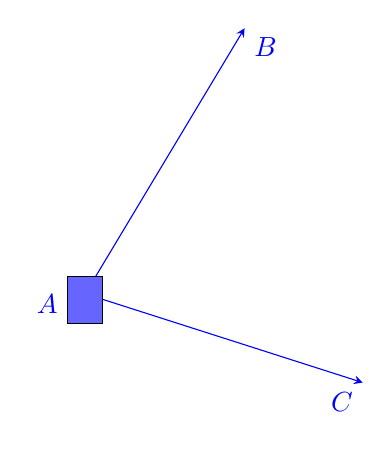
\begin{tikzpicture}[scale=1.5,>=stealth,line join=round,line cap=round]
	\draw[->, blue] (0,0)--(1.5,2.5) node[ below right,scale=1] {$B$};
	\draw[->, blue] (0,0.3)--(2.5,-0.5) node[ below left,scale=1] {$C$};
	\draw[ blue] (0,0) node[ above left,scale=1] {$A$};
	\fill[blue!60] (0,0) rectangle (0.3,0.4);
	\draw (0,0) rectangle (0.3,0.4);
	\end{tikzpicture}}
\loigiai{
Ta có $$AB=\sqrt{(50+10)^2+(30-20)^2}=10\sqrt{37};$$
$$AC=\sqrt{(32+10)^2+(-23-20)^2}=\sqrt{3613};$$
$$BC=\sqrt{(32-50)^2+(-23-30)^2}=\sqrt{3133}.$$
Áp dụng định lí cô-sin trong tam giác $ABC$, ta có
	$$\cos\widehat{BAC}=\dfrac{AB^2+AC^2-BC^2}{2\cdot AB \cdot AC}=\dfrac{3700+3613-3133}{2\cdot 10\sqrt{37}\cdot \sqrt{3613}}\approx 0{,}57 $$ $$ \Rightarrow \widehat{BAC} \approx 55^{\circ}8'.$$
}
\end{ex}

%Câu 32
\begin{ex}%[0D8H1-2]%[Dự án đề kiểm tra Đợt 13 - Toán 10 GHKII NH23-24- VUNgocHao]%[THPT - chuyên Lê Quý Đôn - Ninh Thuận]
	Một chồng sách có $4$ quyển sách Toán và $3$ quyển sách Vật lý, các quyển sách đôi một khác nhau. Hỏi có bao nhiêu cách xếp các quyển sách trên lên kệ sách sao cho $4$ quyển sách Toán xếp cạnh nhau?
	\choice
	{$144$}{$24$}{$120$}{\True $576$}
	\loigiai{
	Xem $4$ quyển sách Toán là $1$ bộ sách. \\
	Khi đó sắp xếp $3$ quyển sách Vật lý và $1$ bộ sách Toán lên kệ sách có $4!=24$ cách. \\
	Sắp xếp $4$ quyển sách Toán có $4!=24$ cách. \\
	Vậy số cách sắp xếp các quyển sách thỏa mãn yêu cầu bài toán là $24\cdot 24=576$ cách.	
	}
\end{ex}

%Câu 33
\begin{ex}%[0D8H1-2]%[Dự án đề kiểm tra Đợt 13 - Toán 10 GHKII NH23-24- VUNgocHao]%[THPT - chuyên Lê Quý Đôn - Ninh Thuận]
	Một hộp có  $6$ viên bi vàng khác nhau và $9$ viên bi xanh khác nhau. Hỏi có bao nhiêu cách chọn $5$ viên bi trong đó có $2$ viên bi vàng?
	\choice
	{$720$}{$15120$}{\True $1260$}{$99$}
	\loigiai{
	Chọn $2$ viên bi vàng từ $6$ viên bi vàng có $\mathrm{C}_{6}^{2}=15$ cách.\\
	Chọn $3$ viên bi xanh từ $9$ viên bi xanh có $\mathrm{C}_{9}^{3}=84$ cách.\\
	Vậy số cách chọn ra $5$ viên bi trong đó có $2$ viên bi vàng là $15\cdot 84=1260$ cách.	
	}
\end{ex}


%Câu 34
\begin{ex}%[0D8V1-2]%[Dự án đề kiểm tra Đợt 13 - Toán 10 GHKII NH23-24- VUNgocHao]%[THPT - chuyên Lê Quý Đôn - Ninh Thuận]
	Bạn Lan chọn mật khẩu cho tài khoản Facebook của mình gồm $8$ kí tự, trong đó $3$ kí tự đầu tiên là ba chữ cái in thường đôi một khác nhau, $2$ kí tự tiếp theo là hai chữ cái in hoa đôi một khác nhau (các chữ cái chọn từ bảng chữ cái Tiếng Anh gồm $26$ chữ cái), $2$ kí tự tiếp theo là các chữ số và kí tự cuối cùng là một trong ba kí tự đặc biệt: @, \#, \$. Hỏi bạn Lan có bao nhiêu cách tạo ra một mật khẩu?
	\choice
	{$24640{,}2\cdot 10^{5}$}
	{$27378\cdot 10^{5}$}
	{\True $30420\cdot 10^{5}$}
	{$9126\cdot 10^{5}$}
	\loigiai{
	Chọn $3$ kí tự đầu tiên là các chữ cái in thường đôi một khác nhau có $\mathrm{A}_{26}^{3}=15600$ cách.\\
	Chọn $2$ kí tự tiếp theo là các chữ cái in hoa có $\mathrm{A}_{26}^2=650$ cách.\\
	Chọn $2$ chữ số cho hai kí tự tiếp theo có $10\cdot 10=100$ cách.\\
	Chọn một trong ba kí tự đặc biệt có $3$ cách.\\
	Vậy bạn Lan có $15600\cdot 650\cdot 100\cdot 3=30420\cdot 10^{5}$ (cách).
	}
\end{ex}


%Câu 35
\begin{ex}%[0H9V3-2]%[Dự án đề kiểm tra Đợt 13 - Toán 10 GHKII NH23-24- VUNgocHao]%[THPT - chuyên Lê Quý Đôn - Ninh Thuận]
Theo Google Maps, sân bay Nội Bài có vĩ độ $21{,}2^{\circ}$ Bắc, kinh độ $105{,}8^{\circ}$ Đông; sân bay Cam Ranh có vĩ độ $12^{\circ}$ Bắc, kinh độ $109{,}2^{\circ}$  Đông. Một máy bay, bay thẳng từ sân bay Nội Bài đến sân bay Cam Ranh. Tại thời điểm $t$ giờ, tính từ lúc xuất phát, máy bay ở vị trí có vĩ độ $x^\circ$  Bắc, kinh độ $y^\circ$ Đông được tính theo công thức:
\begin{center}
	$\heva{&x=21,2 -\dfrac{276}{65}t\\
		&y=105{,}8+\dfrac{102}{65}t.}$
\end{center}
Chuyến bay từ Nội Bài đến Cam Ranh mất $t_{0}$ giờ, $t_{0}$ thuộc khoảng nào sau đây?
	\choice
	{$(1;2)$}{$(3;4)$}{\True $(2;3)$}{$(0;1)$}
	\loigiai{
	Ở thời điểm $t_0=0$ thì máy bay ở Hà Nội với tọa độ $(21{,}2;105{,}8)$.\\
	Khi máy bay xuống sân bay Cam Ranh, máy bay sẽ có tọa độ $(12;109{,}2)$.\\
	Ta có $$\heva{&12=21{,}2-\dfrac{276}{65}t\\
		&109{,}2=105{,}8+\dfrac{102}{65}t} \Leftrightarrow \heva{&-9{,}2=\dfrac{276}{65}t\\
		&3{,}4=\dfrac{102}{65}t} \Leftrightarrow \heva{&t=\dfrac{13}{6}\\
		&t=\dfrac{13}{6}} \Rightarrow t=\dfrac{13}{6} \in (2;3).$$
	
	}
\end{ex}



\Closesolutionfile{ans}
\begin{center}
	\textbf{ĐÁP ÁN}
	\inputansbox{10}{ans/anskq}	
\end{center}
\begin{center}
	\textbf{PHẦN 2 - TỰ LUẬN}
\end{center}

%Câu 1...........................
\begin{ex}%[0D8H1-2]%[Dự án đề kiểm tra Đợt 13 - Toán 10 GHKII NH23-24- VUNgocHao]%[THPT - chuyên Lê Quý Đôn - Ninh Thuận]
Một đội học sinh giỏi của trường THPT \textit{X} gồm $5$ học sinh khối $12$, $4$ học sinh khối 11 và $3$ học sinh khối $10$. Hỏi có bao nhiêu cách chọn ba học sinh trong đó mỗi khối có một học sinh?
\loigiai{
Chọn $1$ học sinh từ $5$ học sinh khối $5$ có $12$ cách.\\
Chọn $1$ học sinh từ $4$ học sinh khối $11$ có $4$ cách.\\
Chọn $1$ học sinh từ $3$ học sinh khối $10$ có $3$ cách.\\
Vậy số cách chọn ba học sinh trong đó mỗi khối có một học sinh là $5\cdot 4\cdot 3=60$ (cách).
}
\end{ex}

%Câu 2...........................
\begin{ex}%[0H9N3-2]%[0H9V3-6]%[Dự án đề kiểm tra Đợt 13 - Toán 10 GHKII NH23-24- VUNgocHao]%[THPT - chuyên Lê Quý Đôn - Ninh Thuận]
	Trong mặt phẳng tọa độ $Oxy$, cho hai điểm $A(0;2)$ $B(-1;0)$ và đường thẳng \\
	$\Delta\colon \heva{&x=t\\ &y=4+2t.}$\\
\begin{enumerate}
	\item Lập phương trình tổng quát của đường thẳng $AB$. 
	\item  Tìm toạ độ của điểm $H$ thuộc đường thẳng $\Delta$ để tam giác $ABH$ vuông tại $H$.
\end{enumerate}
	\loigiai{
	\begin{enumerate}
		\item Ta có $\vec{AB}=(-1;-2)$.\\
		Phương trình đường thẳng $AB$ đi qua $A(0;2)$ và nhận $\vec{n}=(2;-1)$ làm véc-tơ pháp tuyến có dạng
		\begin{center}
			$2\cdot(x-0)- 1\cdot(y-2)=0 \Leftrightarrow 2x-y+2=0$.
		\end{center}
		\item  Giả sử $H(t;4+2t) \in \Delta$.\\ Ta có $\vec{AH}=(t; 2t+2)$, $\vec{BH}= (t+1; 2t+4)$.\\
		Tam giác $ABH$ vuông tại $H$ khi và chỉ khi 
				\begin{eqnarray*}
				&~&	\vec{AH}\cdot \vec{BH}=0 \\
				&\Leftrightarrow& t\cdot(t+1)+(2t+2)\cdot(2t+4)=0\\
				& \Leftrightarrow & 5t^2+13t+8=0 \\
				& \Leftrightarrow & \hoac{&t=-1\Rightarrow H(-1;2)\\&t=-\dfrac{8}{5}\Rightarrow H\left(-\dfrac{8}{5}; \dfrac{4}{5}\right).}
			\end{eqnarray*}
Vậy có $2$ điểm $H$ thỏa mãn yêu cầu bài toán là $H(-1;2)$ hoặc $H\left(-\dfrac{8}{5}; \dfrac{4}{5}\right)$.
	\end{enumerate}
	}
\end{ex}

%Câu 3...........................
\begin{ex}%[0D8V2-2]%[Dự án đề kiểm tra Đợt 13 - Toán 10 GHKII NH23-24- VUNgocHao]%[THPT - chuyên Lê Quý Đôn - Ninh Thuận]
Một nhóm công nhân gồm $14$ nam và $6$ nữ. Người ta muốn chọn từ nhóm ra $5$ người để lập thành một tổ công tác sao cho phải có $1$ tổ trưởng nam, $1$ tổ phó nam và có ít nhất $1$ tổ viên là nữ. Hỏi có bao nhiêu cách lập tổ công tác?
	\loigiai{
{\bf	Bước 1:} Chọn ra $2$ nam từ $14$ nam để xếp vào hai vị trí tổ trưởng, tổ phó có $\mathrm{A}_{14}^{2}=182$ cách.\\
{\bf	Bước 2:} Chọn 3 công nhân còn lại sao cho có ít nhất $1$ tổ viên là nữ.
\begin{itemize}
	\item TH1: Chọn ra $1$ nữ từ $6$ nữ và $2$ nam từ $12$ nam còn lại có $\mathrm{C}_{6}^1\cdot \mathrm{C}_{12}^2=396$ cách.
	\item TH2: Chọn ra $2$ nữ từ $6$ nữ và $1$ nam từ $12$ nam còn lại có $\mathrm{C}_{6}^2\cdot \mathrm{C}_{12}^1=180$ cách.
	\item TH3: Chọn ra $3$ nữ từ $6$ nữ có $\mathrm{C}_{6}^3=20$ cách.
\end{itemize}
Vậy số cách chọn thỏa mãn yêu cầu bài toán là $$182\cdot (396+180+20)=108\,472\, \text{(cách)}.$$

	}
\end{ex}

\begin{center}
	\textbf{--------HẾT--------}
\end{center}
